\section{Supplementary material Section 3}

\begin{figure} 
\centering
    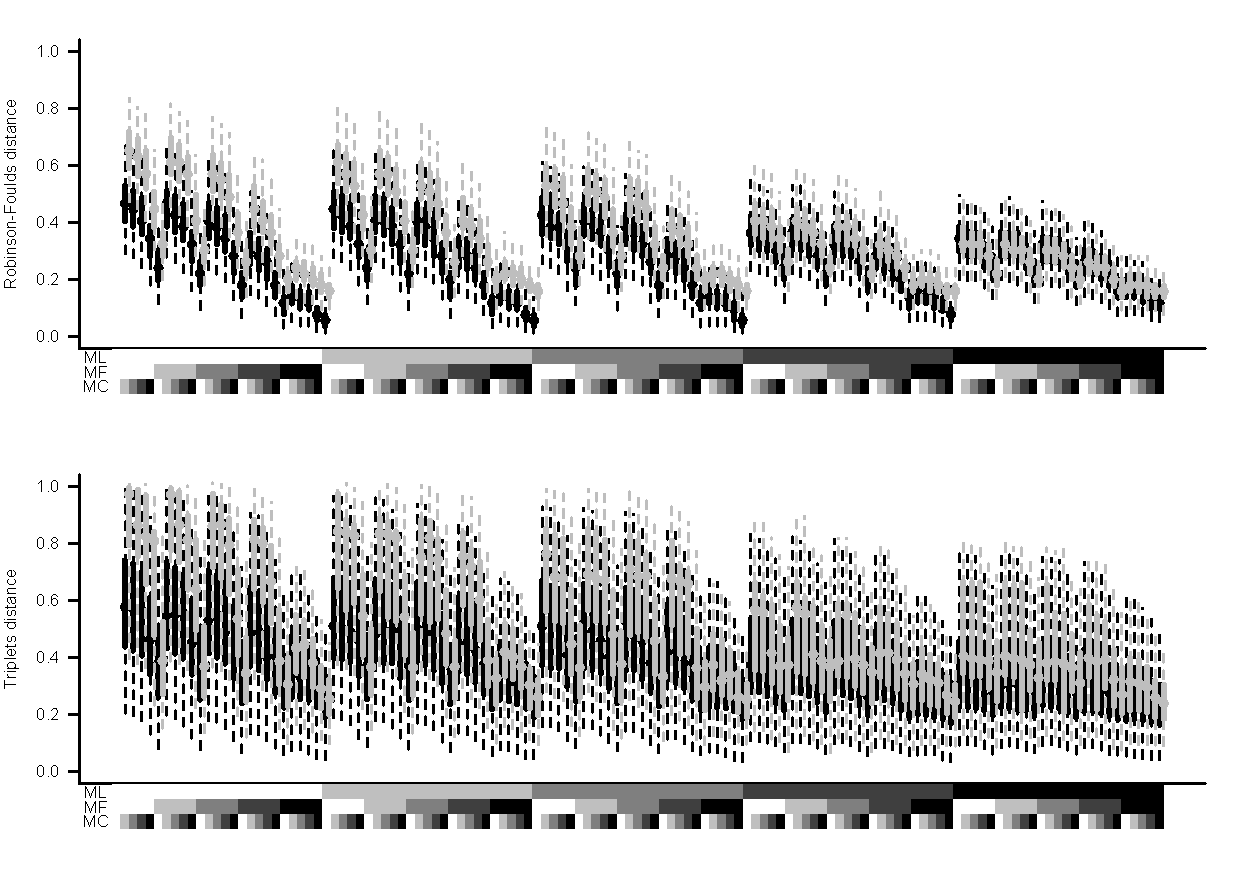
\includegraphics[width=1\textwidth]{SupplementaryMaterial/Supp_Figures/Boot+Baytre-AllParam-RF+Tr.pdf}
\caption{Trend of the effect of missing data on topological recovery on the Bootstraps and the Bayesian posterior trees distributions. The amount of missing data per parameter ($M_{L}$, $M_{F}$ and $M_{C}$) is represented along the x axis. The colour gradient from white to black represents respectively, 0\%, 10\%, 25\%, 50\% and 75\% of missing data. The topological recovery is represented on the y axis, both using Robinson-Foulds distance (upper row) and Triplets distance (lower row). Points represent the modal value of each distribution ; thick solid and thin dashed lines represents respectively the 50\% and 95\% confidence intervals or the distributions. The Bootstraps are represented in black and the Bayesian posterior trees distributions in grey.}
\label{Fig_global_BootTreesets} %Differences between all the parameters and between two methods (Boot vs treesets)
\end{figure}

\begin{figure} 
\centering
    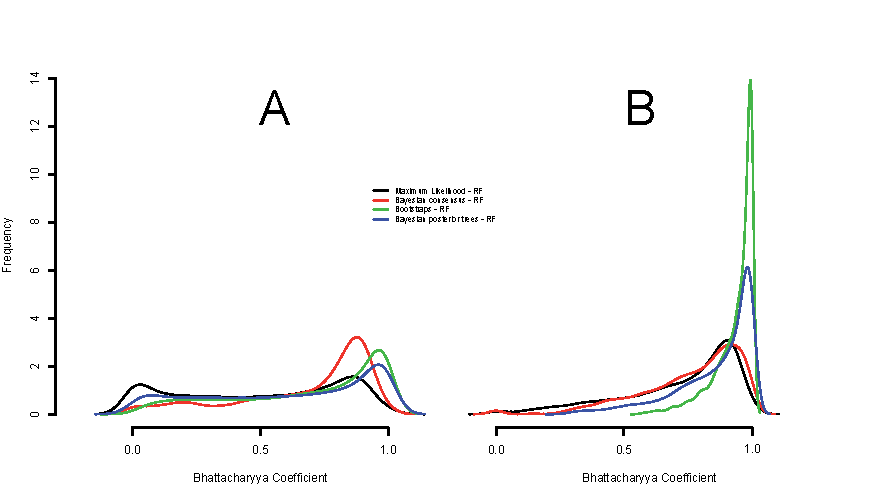
\includegraphics[width=1\textwidth]{SupplementaryMaterial/Supp_Figures/BC-AllMethods-RF+Tr.pdf}
\caption{Distribution of the Pairwise Bhattacharyya Coefficients within each method. A- Distribution of the coefficients when comparing Ronbinson-Foulds distances. B- Distribution of the coefficients when comparing Triplets distances.}
\label{Fig_Bhatt.coeff_distribution} %Differences in overlap within each method
\end{figure}

\begin{figure} 
\centering
    \includegraphics[width=1\textwidth]{SupplementaryMaterial/Supp_Figures/PairwiseComp-ML-RF+Tr.pdf}
\caption{Pairwise Bhattacharyya Coefficients within the Maximum Likelihood trees. The pairwise trees comparisons are represent on both axis. The colour gradient from white to black represents respectively, 0\%, 10\%, 25\%, 50\% and 75\% of missing data for each parameter. The matrix represents the values of pairwise Bhattacharyya Coefficients going from green (1) to red (0). A. Results for the Normalised Robinson-Foulds distance. B. Results with the for Normalised Triplets distance.}
\label{Fig_pairComp-Baytree-RF}
\end{figure} %Pairwise BC for the ML for RF+Tr. (parameters differences)

\begin{figure} 
\centering
    \includegraphics[width=1\textwidth]{SupplementaryMaterial/Supp_Figures/PairwiseComp-Boot-RF+Tr.pdf}
\caption{Pairwise Bhattacharyya Coefficients within the Bootstrap trees. The pairwise trees comparisons are represent on both axis. The colour gradient from white to black represents respectively, 0\%, 10\%, 25\%, 50\% and 75\% of missing data for each parameter. The matrix represents the values of pairwise Bhattacharyya Coefficients going from green (1) to red (0). A. Results for the Normalised Robinson-Foulds distance. B. Results with the for Normalised Triplets distance.}
\label{Fig_pairComp-Baytree-Tr}
\end{figure} %Pairwise BC for the Boot for RF+Tr. (parameters differences)

\begin{figure} 
\centering
    \includegraphics[width=1\textwidth]{SupplementaryMaterial/Supp_Figures/PairwiseComp-Baytre-RF+Tr.pdf}
\caption{Pairwise Bhattacharyya Coefficients within the Bayesian posterior distribution trees. The pairwise trees comparisons are represent on both axis. The colour gradient from white to black represents respectively, 0\%, 10\%, 25\%, 50\% and 75\% of missing data for each parameter. The matrix represents the values of pairwise Bhattacharyya Coefficients going from green (1) to red (0). A. Results for the Normalised Robinson-Foulds distance. B. Results with the for Normalised Triplets distance.}
\label{Fig_pairComp-MLbest-RF}
\end{figure} %Pairwise BC for the Baytre for RF+Tr. (parameters differences)


%Summary of metrics values for all parameters combinations
\begin{table}[ht]
\centering
\begin{tabular}{rrrrrrr}
  \hline
 & Min. & 1st Qu. & Median & Mean & 3rd Qu. & Max. \\ 
  \hline
  Maximum likelihood-RF & 0.06 & 0.26 & 0.40 & 0.41 & 0.50 & 0.95 \\ 
  Maximumlikelihood-Tr & 0.29 & 0.45 & 0.59 & 0.63 & 0.84 & 1.00 \\ 
  Bayesian consensus-RF & 0.69 & 0.71 & 0.72 & 0.76 & 0.79 & 0.96 \\ 
  Bayesian consensus-Tr & -0.28 & -0.11 & 0.17 & 0.19 & 0.37 & 0.98 \\ 
  Bootstraps-RF & 0.06 & 0.18 & 0.27 & 0.26 & 0.34 & 0.46 \\ 
  Bootstraps-Tr & 0.23 & 0.31 & 0.35 & 0.38 & 0.45 & 0.58 \\ 
  Bayesian posterior trees-RF & 0.16 & 0.22 & 0.32 & 0.34 & 0.42 & 0.65 \\ 
  Bayesian posterior trees-Tr & 0.24 & 0.35 & 0.40 & 0.50 & 0.67 & 0.98 \\ 
   \hline
   \hline
\end{tabular}
\end{table}

%Summary of metrics values for the ML parameter
\begin{table}[ht]
\centering
\begin{tabular}{rrrrrrr}
  \hline
 & Min. & 1st Qu. & Median & Mean & 3rd Qu. & Max. \\ 
  \hline
Maximum likelihood-RF & 0.44 & 0.51 & 0.63 & 0.66 & 0.78 & 0.95 \\ 
  Maximumlikelihood-Tr & 0.45 & 0.56 & 0.76 & 0.74 & 0.93 & 0.99 \\ 
  Bayesian consensus-RF & 0.71 & 0.73 & 0.80 & 0.82 & 0.88 & 0.95 \\ 
  Bayesian consensus-Tr & 0.37 & 0.46 & 0.67 & 0.67 & 0.87 & 0.96 \\ 
  Bootstraps-RF & 0.34 & 0.37 & 0.42 & 0.41 & 0.44 & 0.46 \\ 
  Bootstraps-Tr & 0.32 & 0.40 & 0.51 & 0.46 & 0.51 & 0.57 \\ 
  Bayesian posterior trees-RF & 0.33 & 0.41 & 0.52 & 0.50 & 0.60 & 0.65 \\ 
  Bayesian posterior trees-Tr & 0.41 & 0.56 & 0.76 & 0.71 & 0.84 & 0.98 \\ 
   \hline
\end{tabular}
\end{table}

%Summary of metrics values for the ML parameter
\begin{table}[ht]
\centering
\begin{tabular}{rrrrrrr}
  \hline
 & Min. & 1st Qu. & Median & Mean & 3rd Qu. & Max. \\ 
  \hline
Maximum likelihood-RF & 0.23 & 0.46 & 0.64 & 0.61 & 0.79 & 0.93 \\ 
  Maximumlikelihood-Tr & 0.65 & 0.84 & 0.95 & 0.89 & 0.99 & 1.00 \\ 
  Bayesian consensus-RF & 0.72 & 0.77 & 0.86 & 0.85 & 0.94 & 0.96 \\ 
  Bayesian consensus-Tr & -0.16 & 0.19 & 0.63 & 0.52 & 0.96 & 0.98 \\ 
  Bootstraps-RF & 0.14 & 0.30 & 0.40 & 0.35 & 0.45 & 0.46 \\ 
  Bootstraps-Tr & 0.37 & 0.49 & 0.54 & 0.51 & 0.56 & 0.57 \\ 
  Bayesian posterior trees-RF & 0.24 & 0.45 & 0.57 & 0.51 & 0.63 & 0.65 \\ 
  Bayesian posterior trees-Tr & 0.44 & 0.81 & 0.86 & 0.82 & 0.98 & 0.98 \\ 
   \hline
\end{tabular}
\end{table}

%Summary of metrics values for the MC parameter
\begin{table}[ht]
\centering
\begin{tabular}{rrrrrrr}
  \hline
 & Min. & 1st Qu. & Median & Mean & 3rd Qu. & Max. \\ 
  \hline
Maximum likelihood-RF & 0.40 & 0.50 & 0.64 & 0.65 & 0.79 & 0.94 \\ 
  Maximumlikelihood-Tr & 0.70 & 0.84 & 0.93 & 0.89 & 0.99 & 1.00 \\ 
  Bayesian consensus-RF & 0.76 & 0.79 & 0.86 & 0.86 & 0.92 & 0.96 \\ 
  Bayesian consensus-Tr & 0.05 & 0.16 & 0.53 & 0.50 & 0.87 & 0.92 \\ 
  Bootstraps-RF & 0.25 & 0.34 & 0.42 & 0.38 & 0.45 & 0.46 \\ 
  Bootstraps-Tr & 0.38 & 0.47 & 0.55 & 0.51 & 0.57 & 0.58 \\ 
  Bayesian posterior trees-RF & 0.32 & 0.44 & 0.58 & 0.52 & 0.62 & 0.65 \\ 
  Bayesian posterior trees-Tr & 0.39 & 0.78 & 0.82 & 0.79 & 0.98 & 0.98 \\ 
   \hline
\end{tabular}
\end{table}


%Summary of the BC between pairs of methods for the ML parameter
\begin{table}[ht]
\centering
\begin{tabular}{rrrrrrr}
  \hline
 & Min. & 1st Qu. & Median & Mean & 3rd Qu. & Max. \\ 
  \hline
Maximum.likelihood.vs..Bayesian.consensus...RF & 0.30 & 0.31 & 0.69 & 0.61 & 0.77 & 1.00 \\ 
  Maximum.likelihood.vs..Bayesian.consensus...Tr & 0.79 & 0.81 & 0.84 & 0.86 & 0.85 & 1.00 \\ 
  Maximum.likelihood.vs..Bootstraps...RF & 0.03 & 0.22 & 0.29 & 0.36 & 0.54 & 0.69 \\ 
  Maximum.likelihood.vs..Bootstraps...Tr & 0.08 & 0.42 & 0.53 & 0.51 & 0.74 & 0.78 \\ 
  Maximum.likelihood.vs..Bayesian.posterior.trees...RF & 0.02 & 0.49 & 0.61 & 0.51 & 0.67 & 0.74 \\ 
  Maximum.likelihood.vs..Bayesian.posterior.trees...Tr & 0.21 & 0.61 & 0.70 & 0.63 & 0.81 & 0.81 \\ 
  Bayesian.consensus.vs..Bootstraps...RF & 0.01 & 0.02 & 0.02 & 0.02 & 0.03 & 0.04 \\ 
  Bayesian.consensus.vs..Bootstraps...Tr & 0.08 & 0.69 & 0.78 & 0.64 & 0.79 & 0.84 \\ 
  Bayesian.consensus.vs..Bayesian.posterior.trees...RF & 0.01 & 0.02 & 0.02 & 0.04 & 0.08 & 0.09 \\ 
  Bayesian.consensus.vs..Bayesian.posterior.trees...Tr & 0.21 & 0.74 & 0.75 & 0.68 & 0.84 & 0.87 \\ 
  Boostraps.vs..Bayesian.posterior.trees...RF & 0.69 & 0.75 & 0.85 & 0.85 & 0.95 & 1.00 \\ 
  Boostraps.vs..Bayesian.posterior.trees...Tr & 0.91 & 0.92 & 0.96 & 0.95 & 0.97 & 0.98 \\ 
   \hline
\end{tabular}
\end{table}

%Summary of the BC between pairs of methods for the MF parameter
\begin{table}[ht]
\centering
\begin{tabular}{rrrrrrr}
  \hline
 & Min. & 1st Qu. & Median & Mean & 3rd Qu. & Max. \\ 
  \hline
Maximum.likelihood.vs..Bayesian.consensus...RF & 0.00 & 0.25 & 0.48 & 0.50 & 0.76 & 1.00 \\ 
  Maximum.likelihood.vs..Bayesian.consensus...Tr & 0.38 & 0.69 & 0.75 & 0.72 & 0.80 & 1.00 \\ 
  Maximum.likelihood.vs..Bootstraps...RF & 0.03 & 0.18 & 0.32 & 0.36 & 0.47 & 0.77 \\ 
  Maximum.likelihood.vs..Bootstraps...Tr & 0.08 & 0.34 & 0.40 & 0.38 & 0.53 & 0.55 \\ 
  Maximum.likelihood.vs..Bayesian.posterior.trees...RF & 0.02 & 0.47 & 0.71 & 0.60 & 0.86 & 0.94 \\ 
  Maximum.likelihood.vs..Bayesian.posterior.trees...Tr & 0.21 & 0.54 & 0.62 & 0.56 & 0.64 & 0.80 \\ 
  Bayesian.consensus.vs..Bootstraps...RF & 0.00 & 0.00 & 0.01 & 0.01 & 0.01 & 0.03 \\ 
  Bayesian.consensus.vs..Bootstraps...Tr & 0.08 & 0.38 & 0.54 & 0.49 & 0.70 & 0.75 \\ 
  Bayesian.consensus.vs..Bayesian.posterior.trees...RF & 0.00 & 0.02 & 0.02 & 0.02 & 0.04 & 0.04 \\ 
  Bayesian.consensus.vs..Bayesian.posterior.trees...Tr & 0.21 & 0.29 & 0.66 & 0.54 & 0.72 & 0.82 \\ 
  Boostraps.vs..Bayesian.posterior.trees...RF & 0.69 & 0.69 & 0.72 & 0.71 & 0.72 & 0.72 \\ 
  Boostraps.vs..Bayesian.posterior.trees...Tr & 0.91 & 0.91 & 0.91 & 0.93 & 0.92 & 0.98 \\ 
   \hline
\end{tabular}
\end{table}

%Summary of the BC between pairs of methods for the MC parameter
\begin{table}[ht]
\centering
\begin{tabular}{rrrrrrr}
  \hline
 & Min. & 1st Qu. & Median & Mean & 3rd Qu. & Max. \\ 
  \hline
Maximum.likelihood.vs..Bayesian.consensus...RF & 0.03 & 0.32 & 0.66 & 0.55 & 0.75 & 1.00 \\ 
  Maximum.likelihood.vs..Bayesian.consensus...Tr & 0.51 & 0.69 & 0.80 & 0.76 & 0.80 & 1.00 \\ 
  Maximum.likelihood.vs..Bootstraps...RF & 0.03 & 0.17 & 0.21 & 0.31 & 0.46 & 0.68 \\ 
  Maximum.likelihood.vs..Bootstraps...Tr & 0.08 & 0.31 & 0.39 & 0.39 & 0.56 & 0.61 \\ 
  Maximum.likelihood.vs..Bayesian.posterior.trees...RF & 0.02 & 0.44 & 0.47 & 0.52 & 0.78 & 0.90 \\ 
  Maximum.likelihood.vs..Bayesian.posterior.trees...Tr & 0.21 & 0.52 & 0.59 & 0.55 & 0.66 & 0.77 \\ 
  Bayesian.consensus.vs..Bootstraps...RF & 0.00 & 0.01 & 0.01 & 0.02 & 0.02 & 0.03 \\ 
  Bayesian.consensus.vs..Bootstraps...Tr & 0.08 & 0.47 & 0.62 & 0.51 & 0.66 & 0.73 \\ 
  Bayesian.consensus.vs..Bayesian.posterior.trees...RF & 0.00 & 0.02 & 0.04 & 0.04 & 0.05 & 0.06 \\ 
  Bayesian.consensus.vs..Bayesian.posterior.trees...Tr & 0.21 & 0.45 & 0.64 & 0.57 & 0.74 & 0.79 \\ 
  Boostraps.vs..Bayesian.posterior.trees...RF & 0.69 & 0.73 & 0.73 & 0.76 & 0.81 & 0.86 \\ 
  Boostraps.vs..Bayesian.posterior.trees...Tr & 0.91 & 0.92 & 0.93 & 0.94 & 0.96 & 0.99 \\ 
   \hline
\end{tabular}
\end{table}